\documentclass[18pt]{beamer}
\usetheme{Madrid}

\usepackage{graphics}
\usepackage{listings}
\usepackage{url}

\definecolor{listcomment}{rgb}{0.0,0.5,0.0}
\definecolor{listkeyword}{rgb}{0.0,0.0,0.5}
\definecolor{listnumbers}{gray}{0.65}
\definecolor{listlightgray}{gray}{0.955}
\definecolor{listwhite}{gray}{1.0}
\definecolor{listbackground}{rgb}{0.9,0.9,1.0}


\lstset{language=C++}
\lstset{numbers=left}
\lstset{frame=tb}
\lstset{xleftmargin=0.05\linewidth}
\lstset{backgroundcolor=\color{listbackground}}
\lstset{basicstyle=\tiny}
\lstset{keywordstyle=\color{listkeyword}\bfseries}
\lstset{identifierstyle=\color{blue}}
\lstset{commentstyle=\color{listcomment}}
\lstset{stringstyle=\ttfamily\color{red}}
\lstset{showstringspaces=false}


\newcommand{\centeredlargetext}[3]{
{
\setbeamertemplate{navigation symbols}{}
\setbeamercolor{background canvas}{bg={#1}}
\color{#2}
\begin{frame}[plain]
\fontsize{36pt}{36pt}\selectfont
\center
\begin{center}
{#3}
\end{center}
\end{frame}
}}

\newcommand{\centeredhugetext}[3]{
{
\setbeamertemplate{navigation symbols}{}
\setbeamercolor{background canvas}{bg={#1}}
\fontsize{72pt}{72pt}\selectfont
\color{#2}
\begin{frame}[plain]
\center
\begin{center}
{#3}
\end{center}
\end{frame}
}}


\begin{document}

\title[ITK - OpenCV]{ITK Meets OpenCV}
\subtitle[ITK-OpenCV]{A New Open Source Software Resource for CV}
\institute[Insight Software Consortium]{Insight Software Consortium}
\date[June 2011]{June 2011}

\begin{frame}
\titlepage
\end{frame}


{
\setbeamertemplate{navigation symbols}{}
\begin{frame}[plain]
\center
\begin{center}
This presentation is copyrighted by\\
The \textbf{Insight Software Consortium}\\
\bigskip
distributed under the\\
\textbf{Creative Commons by Attribution License 3.0}\\
\url{http://creativecommons.org/licenses/by/3.0}\\
\bigskip
Images used in this presentation are attributed in the last slide.
\end{center}
\end{frame}
}


\begin{frame}
  \tableofcontents
\end{frame}


\begin{frame}
\frametitle{What this Tutorial is about}
\framesubtitle{Amitha to do this}
\begin{itemize}
\item Goals of the tutorial
\item 
\end{itemize}
\end{frame}


\begin{frame}
\frametitle{Program}
\begin{itemize}
\item Virtual Machines Preparation (15min)
\pause
\item ITK Overview (30min)
\pause
\item Software Environment (15min)
\pause
\item ITK Introduction (30min)
\pause
\item OpenCV Introduction (30min)
\pause
\item OpenCV+ITK (30min)
\pause
\item ITK Integration in C++ Applications (30min)
\pause
\item ITK Video Filters (60min)
\end{itemize}
\end{frame}


\section{Virtual Machines Preparation}

\centeredlargetext{white}{black}{
Virtual Machines Preparation
}

\begin{frame}
\frametitle{Virtual Machines Preparation}
\begin{itemize}
\item Get USB Memory Stick
\pause
\item Install VirtualBox from it
\pause
\item Import the VirtualMachine file
\pause
\item Boot the Virtual Machine
\pause
\item Log in
\pause
\item Get familiar with directories
\end{itemize}
\end{frame}


\begin{frame}
\frametitle{USB Memory Stick Content}
\framesubtitle{Directories and Files}
\begin{itemize}
\item VirtualBoxInstallers
\begin{itemize}
\item VirtualBox-4.0.8-71778-OSX.dmg (Mac)
\item VirtualBox-4.0.8-71778-Win.exe (Windows)
\item (Ubuntu Linux)
\begin{itemize}
\item virtualbox-4.0\_4.0.8-71778~Ubuntu~lucid\_amd64.deb
\item virtualbox-4.0\_4.0.8-71778~Ubuntu~lucid\_i386.deb
\item virtualbox-4.0\_4.0.8-71778~Ubuntu~maverick\_amd64.deb
\item virtualbox-4.0\_4.0.8-71778~Ubuntu~maverick\_i386.deb
\item virtualbox-4.0\_4.0.8-71778~Ubuntu~natty\_amd64.deb
\item virtualbox-4.0\_4.0.8-71778~Ubuntu~natty\_i386.deb
\item \ldots
\end{itemize}
\end{itemize}
\pause
\item VirtualMachine
\begin{itemize}
\item  "{859d59f9-ed19-4aa2-9cd6-a852ba47cdac}.vmdk"
\item  "OpenCV-ITK.ovf"
\end{itemize}
\end{itemize}
\end{frame}

\begin{frame}
\frametitle{Install VirtualBox}
\begin{itemize}
\item Select the installer for your platform
\item Run it
\end{itemize}
\end{frame}

\begin{frame}
\frametitle{Alternative Linux Installation}
\begin{itemize}
\item  You can also install VirtualBox by doing:
\item  sudo apt-get install virtualbox-ose-qt
\end{itemize}
\end{frame}

\begin{frame}
\frametitle{Importing the Virtual Machine}
\begin{itemize}
\item Run VirtualBox
\item In ``File'' Menu select ``Import Appliance''
\item Provide the filename in the USB stick "VirtualMachine/OpenCV-ITK.ovf"
\item A progress bar will appear, and when it finishes you should see:
\end{itemize}
\begin{center}
  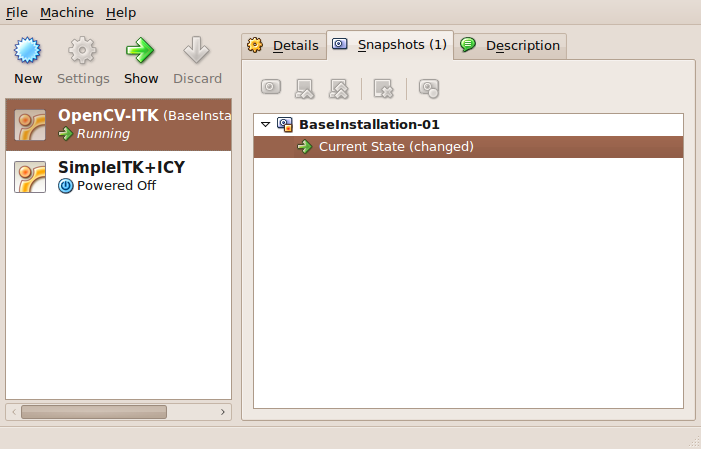
\includegraphics[width=0.5\paperwidth]{Screenshot-VirtualBox-OSE-01.png}
\end{center}
\end{frame}

\begin{frame}
\frametitle{Booting the Virtual Machine}
\begin{itemize}
\item Click on the ``OpenCV-ITK'' icon on the left, to select it.
\item Click on the Green Arrow at the top ``Show''.
\item The VM will start to boot and you will see the warning:
\end{itemize}
\begin{center}
  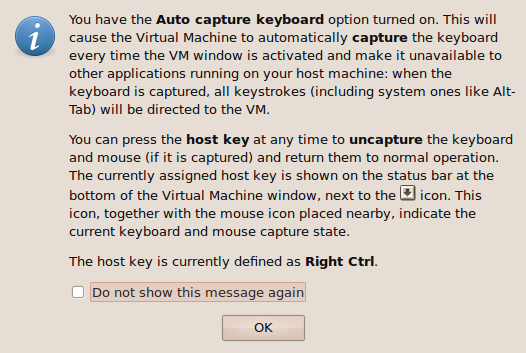
\includegraphics[width=0.4\paperwidth]{Screenshot-VirtualBox-OSE-02.png}
\end{center}
\begin{itemize}
\item Click ``OK''
\end{itemize}
\end{frame}

\begin{frame}
\frametitle{Booting the Virtual Machine}
\begin{itemize}
\item The boot sequence should continue and you shold see:
\end{itemize}
\begin{center}
  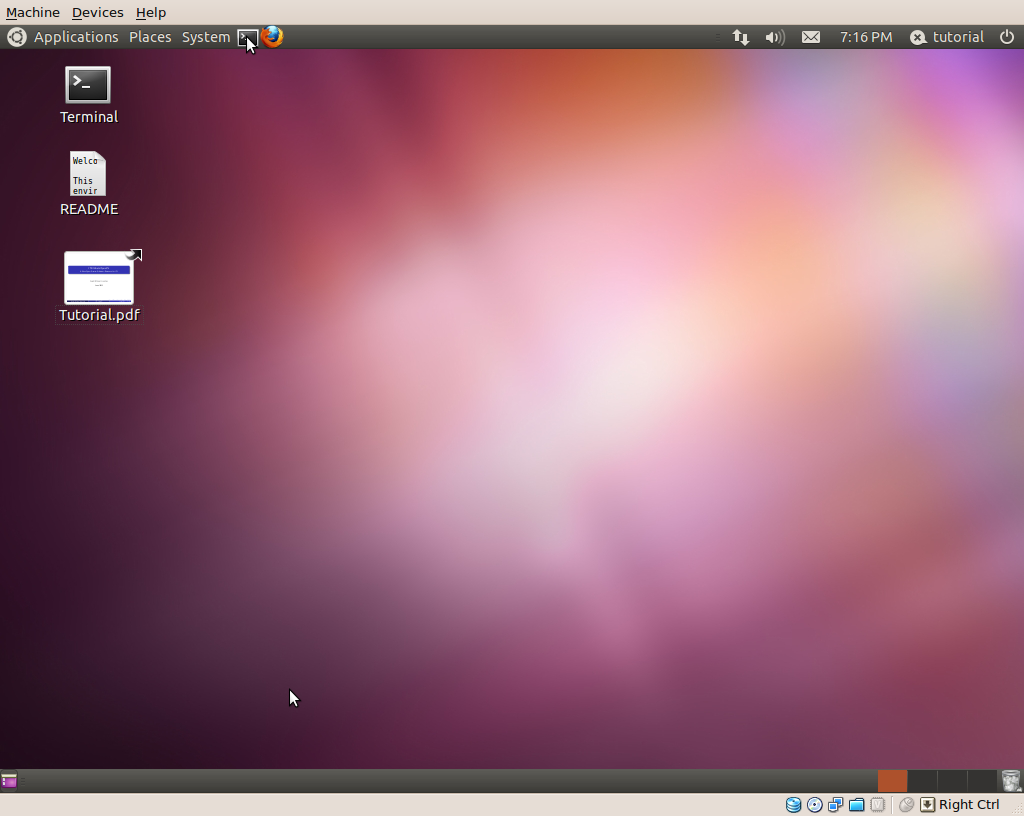
\includegraphics[width=0.7\paperwidth]{Screenshot-OpenCV-ITK-VirtualBox-01.png}
\end{center}
\end{frame}

\centeredlargetext{white}{black}{
Your Virtual Machine\\ is Ready !
}

\begin{frame}
\frametitle{Additional Copies}
\begin{itemize}
\item The same source trees are available in the USB key
\item Outside of the VirtualBox image
\end{itemize}
\end{frame}



\section{ITK Overview}


\centeredlargetext{white}{black}{
ITK Overview
}

\begin{frame}[fragile]
\frametitle{The Insight Toolkit (ITK)}
\begin{center}
  
\includegraphics[width=0.5\paperwidth]{itkLogo.png}
\end{center}
\end{frame}

\begin{frame}
\frametitle{What is ITK ?}
\begin{itemize}
\item C++ Library
\pause
\item Open Source (Apache 2.0 License)
\pause
\item Generic Programming / C++ Templates
\pause
\item Image Processing
\pause
\item Image Segmentation
\pause
\item Image Registration
\end{itemize}
\end{frame}


\begin{frame}
\frametitle{What ITK is not ?}
\begin{itemize}
\item No Visualization
\pause
\item No GUI
\end{itemize}
\end{frame}

\begin{frame}
\frametitle{Funding}
\begin{itemize}
\item Funded (mostly) by the US National Library of Medicine
\pause
\item With contributions from
\begin{itemize}
\item National Institute of Dental and Craniofacial Research
\item National Science Foundation
\item National Eye Institute
\item National Institute of Neurological Disorders and Stroke
\item National Institute of Mental Health
\item National Institute on Deafness and Other Communication Disorders
\item National Cancer Institute
\end{itemize}
\end{itemize}
\end{frame}

\begin{frame}
\frametitle{History}
\begin{itemize}
\item Started in 2000
\pause
\item Developed by Companies and Universities
\begin{itemize}
\item GE Corporate Research
\item Insightful
\item Kitware
\item UNC Chapel Hill
\item University of Pennsylvania
\item University of Utah
\end{itemize}
\end{itemize}
\end{frame}

\begin{frame}
\frametitle{History}
\begin{itemize}
\item Recent contributions by a larger community
\begin{itemize}
\item Harvard - Brigham and Women's Hospital
\item University of Iowa
\item Georgetown University
\item INRA - France
\item German Cancer Research Center
\item \ldots and many others \ldots
\end{itemize}
\end{itemize}
\end{frame}

\begin{frame}
\frametitle{Project Profile}
\begin{itemize}
\item Total lines of code: 1,886,674
\item Active developers: 56 (past 12 months)
\item Total developers: 146 (full history of the project)
\item Top 2\% largest open source teams in the world
\item Estimated cost of development: \$34.5 M\footnote{Ohloh: \url{http://www.ohloh.net/p/itk}}
\end{itemize}
\end{frame}

\begin{frame}
\frametitle{Funding}
\begin{itemize}
\item First 10 years of development = \$15M
\pause
\item Refactoring of ITKv4 in 2011 = \$5M
\pause
\item Yearly maintenance supported by NLM
\end{itemize}
\end{frame}


\begin{frame}
\frametitle{ITK by the Numbers}
\begin{itemize}
\item Community Size
\pause
\begin{itemize}
\item Users Mailing List
\pause
\begin{itemize}
\item 2,071 Subscribers
\item About 400 emails/month
\end{itemize}
\end{itemize}
\pause
\begin{itemize}
\item Developers Mailing List
\begin{itemize}
\item 475 Subscribers
\item About 350 emails/month
\end{itemize}
\end{itemize}
\pause
\begin{itemize}
\item 4,800 Downloads/month
\pause
\begin{itemize}
\item from 116 countries
\end{itemize}
\end{itemize}
\end{itemize}
\end{frame}

\begin{frame}
\frametitle{What ITK has to offer}
\begin{itemize}
\item Image Processing
\pause
\item Segmentation
\pause
\item Registration
\end{itemize}
\end{frame}

\begin{frame}
\frametitle{Image Processing}
\begin{itemize}
\item Anisotropic Diffusion
\pause
\item Mathematical Morphology
\pause
\item Anti-Aliasing
\pause
\item Resampling
\pause
\item Distance Maps
\pause
\item Bias Correction
\pause
\item Diffussion Tensor Imaging
\pause
\item Hessians, Laplacian, Gaussians
\pause
\item Hough, Canny
\end{itemize}
\end{frame}

\begin{frame}
\frametitle{Image Segmentation}
\begin{itemize}
\item Leve Sets
\pause
\item Region Growing
\pause
\item Watersheds
\pause
\item Label Voting
\pause
\item Connected Components
\pause
\item Label Image Processing
\pause
\item Deformable Models
\pause
\item Cellular Models
\pause
\item Statistical Classification
\begin{itemize}
\item K-Means
\item Gaussian Mixture Models
\item Markov Random Fields
\end{itemize}
\end{itemize}
\end{frame}

\begin{frame}
\frametitle{Image Registration}
\begin{itemize}
\item Generic Framework
\pause
\begin{itemize}
\item Image Metrics
\item Interpolators
\item Transforms
\item Optimizers
\end{itemize}
\pause
\item Deformable Registration
\pause
\begin{itemize}
\item BSplines (Free-form)
\item Demons
\item Diffeomorphic Demons
\item PDE Solving
\end{itemize}
\pause
\item Multi-Resolution
\pause
\item Multi-Modality
\end{itemize}
\end{frame}

\begin{frame}
\frametitle{The Insight Journal}
\framesubtitle{New Algorithms Every Week\ldots}
\begin{itemize}
\item 2,129 Registered Users
\pause
\item 472 Publications
\pause
\item 834 Open Reviews
\pause
\item Open Access Journal
\pause
\item Reproducible Research (RR)
\end{itemize}
\end{frame}



\section{Software Environment}

\centeredlargetext{white}{black}{
Software Environment
}

\begin{frame}
\frametitle{Welcome to Ubuntu GNU/Linux}
\begin{center}

\includegraphics[height=0.5\paperheight]{Tux.png}

\includegraphics[width=0.5\paperwidth]{blackeubuntulogo.png}
\end{center}
\end{frame}

\begin{frame}
\frametitle{How to take the mouse out of the Virtual Machine}
\begin{itemize}
\item Hit the \textbf{RIGHT CTRL} Key on Windows / Linux Host
\item Hit the \textbf{LEFT APPLE} Key on Mac Host
\end{itemize}
\end{frame}

\begin{frame}
\frametitle{How to Open a Terminal - Icon in Upper Left Corner}
\framesubtitle{To type your command line instructions}
\begin{center}
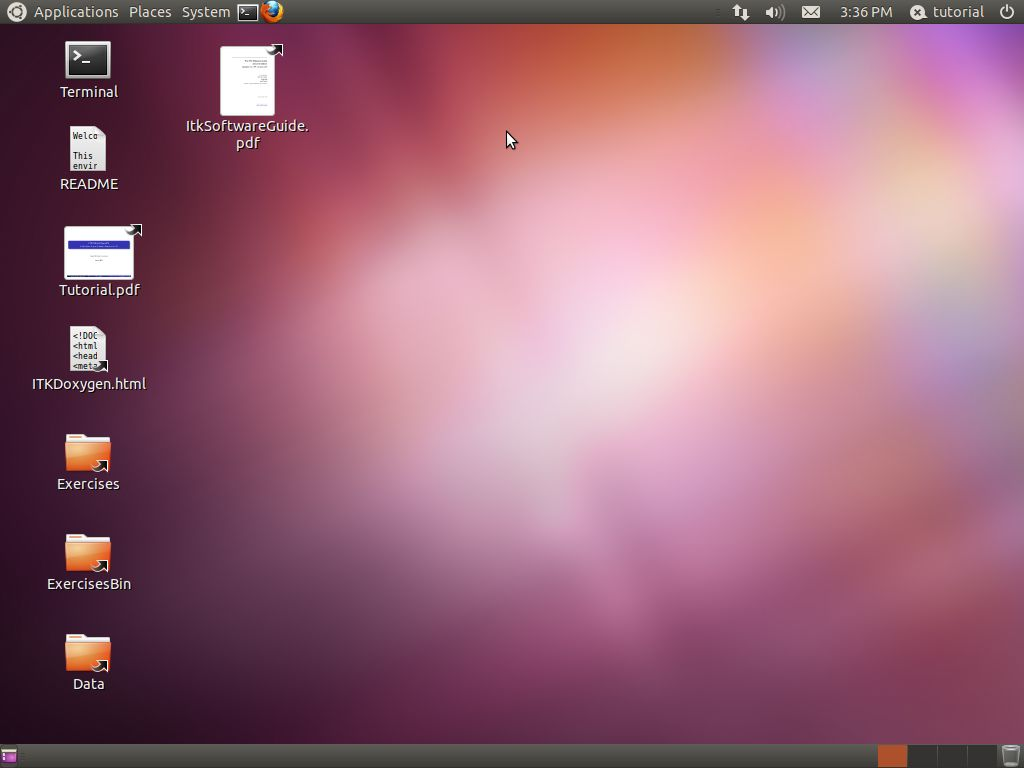
\includegraphics[width=0.7\paperwidth]{Screenshot-OpenTerminal.jpg}
\end{center}
\end{frame}

\begin{frame}
\frametitle{How to Open a Terminal - Icon in Upper Left Corner}
\framesubtitle{To type your command line instructions}
\begin{center}
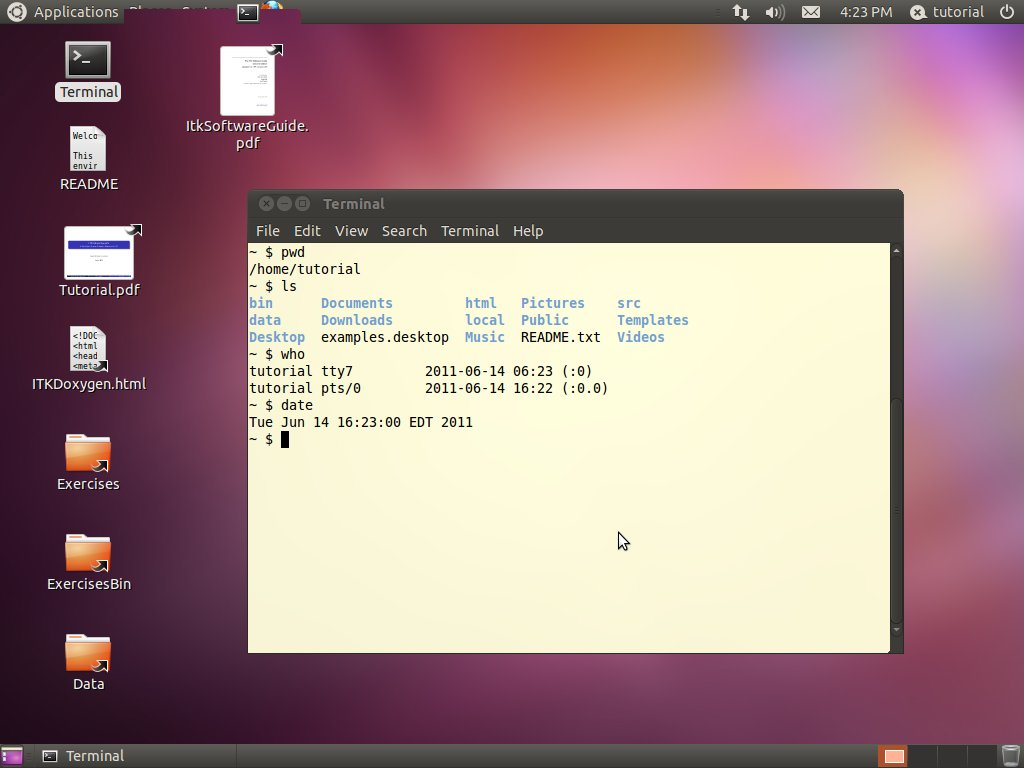
\includegraphics[width=0.7\paperwidth]{Screenshot-Terminal.jpg}
\end{center}
\end{frame}

\begin{frame}
\frametitle{How to Navigate Directories}
\framesubtitle{Double Click in Folder Icons in the Desktop}
\begin{center}
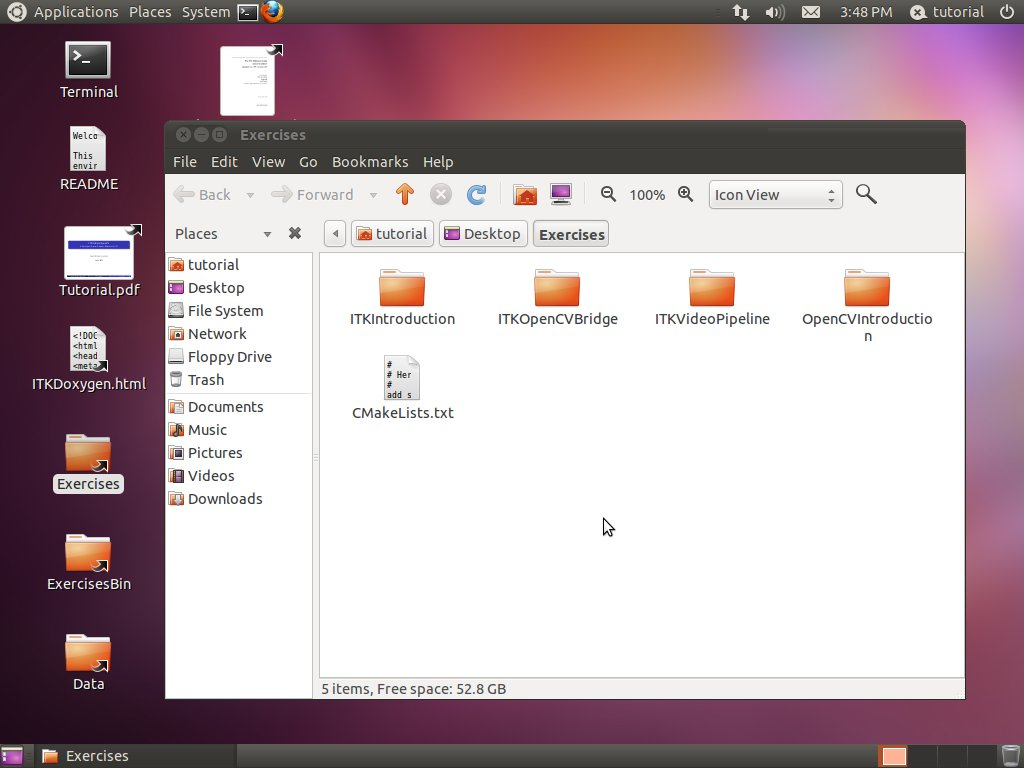
\includegraphics[width=0.7\paperwidth]{Screenshot-Nautilus.jpg}
\end{center}
\end{frame}

\begin{frame}[fragile]
\frametitle{Walk through the directories}
\begin{itemize}
\item Find source code of exercises
\begin{verbatim}
cd ~/src/ITK-OpenCV-Bridge-Tutorial/Exercises
pwd
ls
nautilus .
\end{verbatim}
\pause
\item Find binary build of exercises
\begin{verbatim}
cd ~/bin/ITK-OpenCV-Bridge-Tutorial/Exercises
pwd
ls
\end{verbatim}
\end{itemize}
\end{frame}

\begin{frame}[fragile]
\frametitle{How to View Images}
\begin{itemize}
\item Go to the directory
\item Invoke ``eye of gnome" eog application
\begin{verbatim}
cd ~/data
eog mandrill.png
\end{verbatim}
\pause
\item Hit ESC key to quit the application
\end{itemize}
\end{frame}

\begin{frame}[fragile]
\frametitle{How to View Videos}
\begin{itemize}
\item Go to the directory
\item Invoke ``VideoLAN" vlc application
\begin{verbatim}
cd ~/data
vlc Walk1.mpg
\end{verbatim}
\pause
\item Hit CTRL-Q to quit the application
\item or use the menus
\end{itemize}
\end{frame}


\section{ITK Introduction}


\centeredlargetext{white}{black}{
ITK Introduction
}

\begin{frame}
\frametitle{ITK is a Templated Library}
You will typically do:
\begin{itemize}
\item Include headers
\pause
\item Pick pixel type
\pause
\item Pick image dimension
\pause
\item Instantiate image type
\pause
\item Instantiate filter type
\pause
\item Create filters
\pause
\item Connect pipeline
\pause
\item Run pipeline
\end{itemize}
\end{frame}

{
\setbeamertemplate{navigation symbols}{}
\begin{frame}[fragile]
\frametitle{Basic Filtering}
\framesubtitle{Median Filter}
\begin{itemize}
\item Include headers\footnote{Source code in Exercises/ITKIntroduction/exercise1/BasicImageFilteringITK.cxx}
\end{itemize}
\begin{center}
\lstinputlisting[linerange={19-21}]{BasicImageFilteringITK.cxx}
\end{center}
\pause
\begin{itemize}
\item Read images from files
\item Write images from files
\item Apply a median filter in an image
\end{itemize}
\end{frame}
}

{
\setbeamertemplate{navigation symbols}{}
\begin{frame}[fragile]
\frametitle{Basic Filtering}
\framesubtitle{Median Filter}
\begin{itemize}
\item Declare pixel types and image dimension\footnote{Source code in Exercises/ITKIntroduction/exercise1/BasicImageFilteringITK.cxx}
\end{itemize}
\begin{center}
\lstinputlisting[linerange={32-35}]{BasicImageFilteringITK.cxx}
\end{center}
\pause
\begin{itemize}
\item Declare input and output image types
\end{itemize}
\begin{center}
\lstinputlisting[linerange={37-38}]{BasicImageFilteringITK.cxx}
\end{center}
\end{frame}
}

{
\setbeamertemplate{navigation symbols}{}
\begin{frame}[fragile]
\frametitle{Basic Filtering}
\framesubtitle{Median Filter}
\begin{itemize}
\item Declare the types for reader and writer\footnote{Source code in Exercises/ITKIntroduction/exercise1/BasicImageFilteringITK.cxx}
\end{itemize}
\begin{center}
\lstinputlisting[linerange={40-41}]{BasicImageFilteringITK.cxx}
\end{center}
\pause
\begin{itemize}
\item Instantiate the reader and writer objects (source and sink)
\end{itemize}
\begin{center}
\lstinputlisting[linerange={43-44}]{BasicImageFilteringITK.cxx}
\end{center}
\pause
\begin{itemize}
\item Set input and output filenames
\end{itemize}
\begin{center}
\lstinputlisting[linerange={46-47}]{BasicImageFilteringITK.cxx}
\end{center}
\end{frame}
}

{
\setbeamertemplate{navigation symbols}{}
\begin{frame}[fragile]
\frametitle{Basic Filtering}
\framesubtitle{Median Filter}
\begin{itemize}
\item Declare the Median filter type\footnote{Source code in Exercises/ITKIntroduction/exercise1/BasicImageFilteringITK.cxx}
\end{itemize}
\begin{center}
\lstinputlisting[linerange={49-50}]{BasicImageFilteringITK.cxx}
\end{center}
\pause
\begin{itemize}
\item Create the filter
\end{itemize}
\begin{center}
\lstinputlisting[linerange={51-51}]{BasicImageFilteringITK.cxx}
\end{center}
\end{frame}
}

{
\setbeamertemplate{navigation symbols}{}
\begin{frame}[fragile]
\frametitle{Basic Filtering}
\framesubtitle{Median Filter}
\begin{itemize}
\item Define the Median kernel radius (Manhattan Radius)\footnote{Source code in Exercises/ITKIntroduction/exercise1/BasicImageFilteringITK.cxx}
\end{itemize}
\begin{center}
\lstinputlisting[linerange={55-58}]{BasicImageFilteringITK.cxx}
\end{center}
\pause
\begin{itemize}
\item Connect the pipeline
\end{itemize}
\begin{center}
\lstinputlisting[linerange={60-61}]{BasicImageFilteringITK.cxx}
\end{center}
\end{frame}
}

{
\setbeamertemplate{navigation symbols}{}
\begin{frame}[fragile]
\frametitle{Basic Filtering}
\framesubtitle{Median Filter}
\begin{itemize}
\item Trigger the pipeline execution by calling Update().
\end{itemize}
\begin{center}
\lstinputlisting[linerange={63-71}]{BasicImageFilteringITK.cxx}
\end{center}
\pause
\begin{itemize}
\item ITK uses C++ exceptions for error management
\item Exceptions are typically thrown during Update() calls
\item Applications must catch the exceptions and solve them
\end{itemize}
\end{frame}
}


\begin{frame}
\frametitle{How to Configure and Build}
\framesubtitle{cmake-gui}
\begin{itemize}
\item Create shortcut to build from nautilus
\item Shell script that launches gnome-terminal, cd s to binary dir and user can type "make"
\end{itemize}
\end{frame}


\begin{frame}
\frametitle{Basic Filtering}
\framesubtitle{Replace with Canny Filter}
\begin{center}
\lstinputlisting[linerange={21-23}]{BasicImageFilteringITK.cxx}
\end{center}
\end{frame}


\section{OpenCV Introduction}


\centeredlargetext{white}{black}{
OpenCV Introduction
}


\centeredlargetext{white}{black}{
A Basic Image Filtering Example
}


\begin{frame}
\frametitle{Include Header Files}
\begin{center}
We need to include the OpenCV headers
\lstinputlisting[linerange={19-20}]{BasicFilteringOpenCV.cxx}
\pause
\vspace{1 em}
and standard library headers for {\tt cout} and {\tt string}
\lstinputlisting[linerange={22-23}]{BasicFilteringOpenCV.cxx}
\end{center}

\end{frame}


\begin{frame}
\frametitle{The Main function}
\begin{center}
\lstinputlisting[linerange={26-34,42-45,54-57,60-63}]{BasicFilteringOpenCV.cxx}
\begin{itemize}
\item If no arguments, print usage and exit
\item If one argument, process an image and display the results
\item If two arguments, process an image and save to a file
\end{itemize}
\end{center}

\end{frame}


\begin{frame}
\frametitle{Loading an Image / Applying a Filter}
\begin{center}
\begin{itemize}
\item Load an image from the specified file into a matrix object
\end{itemize}
\lstinputlisting[linerange={36-37}]{BasicFilteringOpenCV.cxx}
\pause
\begin{itemize}
\item Create a matrix for the output and apply a median filter
\end{itemize}
\lstinputlisting[linerange={38-41}]{BasicFilteringOpenCV.cxx}
\end{center}

\end{frame}


\begin{frame}
\frametitle{Displaying an Image}
\begin{center}
\begin{itemize}
\item Use OpenCV HighGUI to display the resulting image
\end{itemize}
\lstinputlisting[linerange={43-54}]{BasicFilteringOpenCV.cxx}
\end{center}
\end{frame}


\begin{frame}
\frametitle{Saving an Image}
\begin{center}
\begin{itemize}
\item Write the image to the specified file
\end{itemize}
\lstinputlisting[linerange={55-60}]{BasicFilteringOpenCV.cxx}
\end{center}
\end{frame}


\begin{frame}[fragile]
\frametitle{Exercise 1}
\begin{center}
\begin{itemize}
\item Replace the median filter with a Canny edge detector
\end{itemize}
\lstinputlisting[numbers=left,linerange={38-41}]{BasicFilteringOpenCV.cxx}
\begin{itemize}
\item Hint: The OpenCV Canny function has this signature
\end{itemize}
\begin{lstlisting}
void Canny(const Mat& image, Mat& edges, double threshold1, double threshold2);
\end{lstlisting}
\begin{itemize}
\item Canny requires grayscale image input, but our images are color
\item Hint: Use this function to convert a color space
\end{itemize}
\begin{lstlisting}
void cvtColor(const Mat& src, Mat& dst, int code);
\end{lstlisting}
\end{center}
\end{frame}


\section{ITK OpenCV Bridge}


\centeredlargetext{white}{black}{
ITK OpenCV Bridge
}

\begin{frame}
\frametitle{Introduction}
\begin{itemize}
\item ITK Module for working with other libraries
\item Moving frame and/or video data between OpenCV and ITK
\item Bring biomedical and computer vision folks together
\item \url{https://github.com/itkvideo/ITK}
\end{itemize}
\end{frame}

\begin{frame}
\frametitle{Funding Source}
\begin{itemize}
\item Contract from the National Library of Medicine (HHSN276201000579P)
\item Algorithms, Adapters \& Data Distribution Outreach 2010:
  Increasing the Impact of the Insight Toolkit (ITK)
\end{itemize}
\end{frame}

\begin{frame}
\frametitle{Design Choices}
\begin{itemize}
\item OpenCV users and ITK users should both be comfortable
\item Image to image utility functions
\item cv::Source to itk::VideoStream
\item (Later) Focus on performance
\end{itemize}
\end{frame}

\centeredlargetext{white}{black}{
Basic Image Filtering (Revisited)
}


\begin{frame}
\frametitle{Include Header Files}
\begin{itemize}
\item We include ITK and OpenCV headers (like before):
\lstlistingwithnumber{21}{21}{Ex1_BasicFilteringOpenCVBridge.cxx}
\lstlistingwithnumber{23}{24}{Ex1_BasicFilteringOpenCVBridge.cxx}
\item We also need to include the bridge header:
\lstlistingwithnumber{25}{25}{Ex1_BasicFilteringOpenCVBridge.cxx}
\end{itemize}
\end{frame}

\begin{frame}
\frametitle{Basic Layout}
\begin{itemize}
\item The basic layout of this file is the same as the OpenCV
  Examples:
\lstlistingwithnumber{28}{36}{Ex1_BasicFilteringOpenCVBridge.cxx}
\lstlistingwithnumber{62}{75}{Ex1_BasicFilteringOpenCVBridge.cxx}
\end{itemize}
\end{frame}

\begin{frame}
\frametitle{Adding ITK}
\begin{itemize}
\item The type definitions should also be familiar from the ITK Material:
\lstinputlisting[linerange={38-45}]{Ex1_BasicFilteringOpenCVBridge.cxx}
\item However, notice the bridge class. It contains the conversion function
between OpenCV and ITK.
\lstlistingwithnumber{43}{43}{Ex1_BasicFilteringOpenCVBridge.cxx}
\end{itemize}
\end{frame}

\begin{frame}
\frametitle{From OpenCV to ITK}
\begin{itemize}
\item We call our conversion function to go from a cv::Mat to an
  itk::Image
\lstlistingwithnumber{47}{48}{Ex1_BasicFilteringOpenCVBridge.cxx}
\end{itemize}
\end{frame}

\begin{frame}
\frametitle{Filtering with ITK}
\begin{itemize}
\item The median filtering is normal ITK code, but we do not connect our
output to a writer
\lstlistingwithnumber{50}{57}{Ex1_BasicFilteringOpenCVBridge.cxx}
\pause
\item Instead, we set it to our conversion function
\lstlistingwithnumber{59}{60}{Ex1_BasicFilteringOpenCVBridge.cxx}
\end{itemize}
\end{frame}

\begin{frame}
\frametitle{Running the Example}
\begin{itemize}
\item Running the example the same way as before, we see a nicely
median-filtered image.
\pause
\item Now, the fun part. Let's modify our example to use Curvature Flow, an
anisotropic diffusion filter built into ITK.
\end{itemize}
\end{frame}

\begin{frame}
\begin{itemize}
\frametitle{Exercise 1}
\item Hint 1: Curvature Flow requires {\tt float} as the pixel
  type.
\pause
\item Hint 2: Curvature Flow does not take a radius parameter. It's
  salient functions are:
\lstlistingwithnumber{49}{50}{Ex1_BasicFilteringOpenCVBridgeAnswer.cxx}
\end{itemize}
\end{frame}

\begin{frame}
\begin{itemize}
\frametitle{Exercise 1 (Answer)}
\item First, change the included filter
\lstlistingwithnumber{23}{23}{Ex1_BasicFilteringOpenCVBridgeAnswer.cxx}
\pause
\item The type definitions also need to change to reflect the new
  filter and output image types.
\lstlistingwithnumber{36}{43}{Ex1_BasicFilteringOpenCVBridgeAnswer.cxx}
\end{itemize}
\end{frame}

\begin{frame}
\begin{itemize}
\frametitle{Exercise 1 (Answer)}
\item The semantics of calling the filter also has to change:
\lstlistingwithnumber{49}{50}{Ex1_BasicFilteringOpenCVBridgeAnswer.cxx}
\pause
\item That's it! Now you're using a ``better'' blurring scheme.
\end{itemize}
\end{frame}

\begin{frame}
\begin{itemize}
\frametitle{Exercise 1 (Answer)}
\item The final pipeline should look like this:
\lstlistingwithnumber{34}{56}{Ex1_BasicFilteringOpenCVBridgeAnswer.cxx}
\end{itemize}
\end{frame}


\section{ITK Integration With Applications}


\centeredlargetext{white}{black}{
ITK Integration With Applications
}





\section{ITK Video Filters}


\centeredlargetext{white}{black}{
ITK Video Filters
}






\end{document}
